\documentclass[]{report}
\usepackage{amsmath}
\usepackage{graphicx}
\usepackage{tabularx}
\usepackage{amsfonts}
\usepackage{amssymb}
\usepackage{amsbsy}

% Title Page
\title{MachineLearning for Visual Computing Aufgabenblock 1}
\author{Christian Br\"andle, Doris Antensteiner}


\begin{document}
\maketitle

%\begin{abstract}
%\end{abstract}

\section{Einfaches Perceptron - Datengeneration}

% Mu_1 = [14,14,14,14]; 
% Sigma_1 = [5,4,3,2];
% Mu_2 = [2, 2, 2, 2]; 
% Sigma_2 = [2,3,4,5];

Gegeben sind vier Datensets a 100 Beobachtungen von 2-dimensionalen Eingangsdaten, welche normalverteilt sind. Die Figuren in Tabelle ~\ref{tab:DataSets} verdeutlichen dies.


\begin{table}[h]
\begin{tabular}{| c | c |}
\hline
 & \\
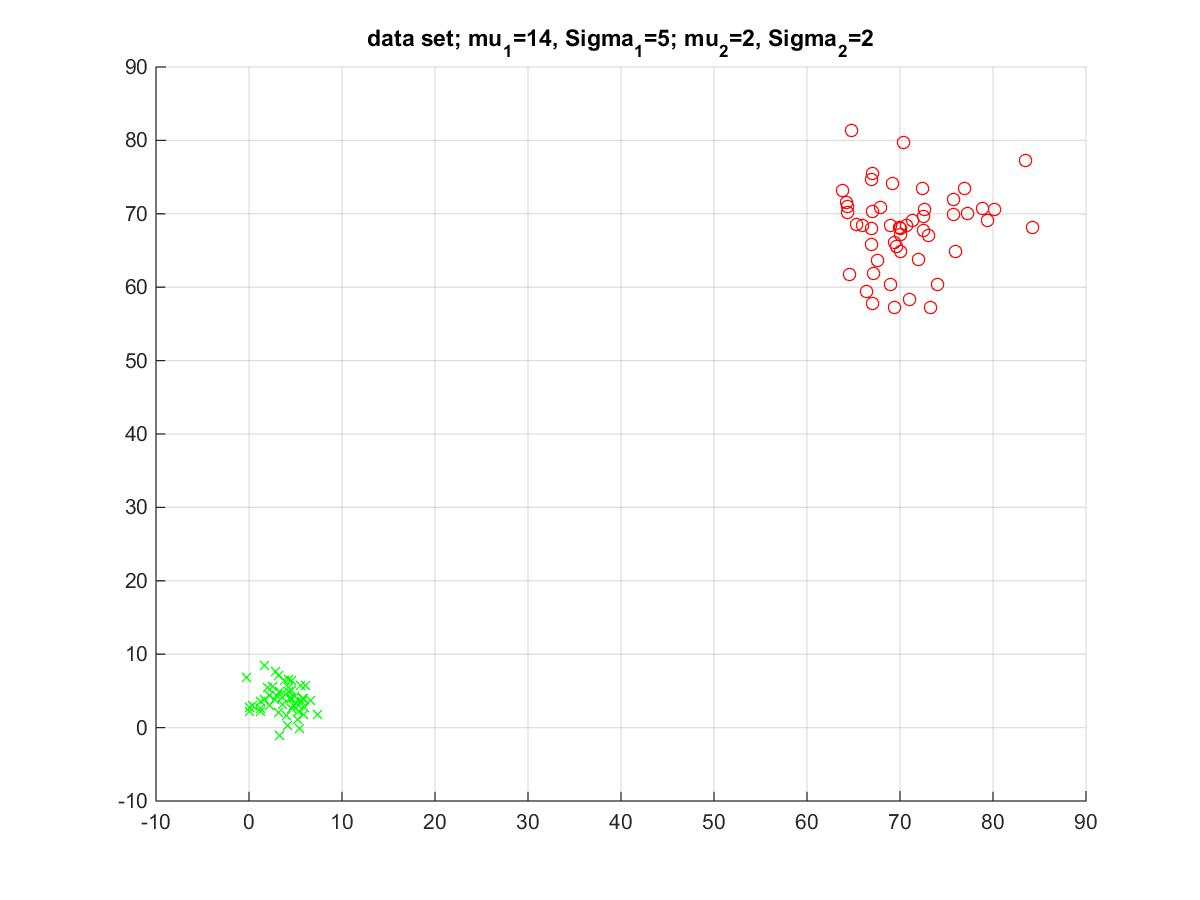
\includegraphics[width=0.4\textwidth]{./images/DataSet_100.jpg} & 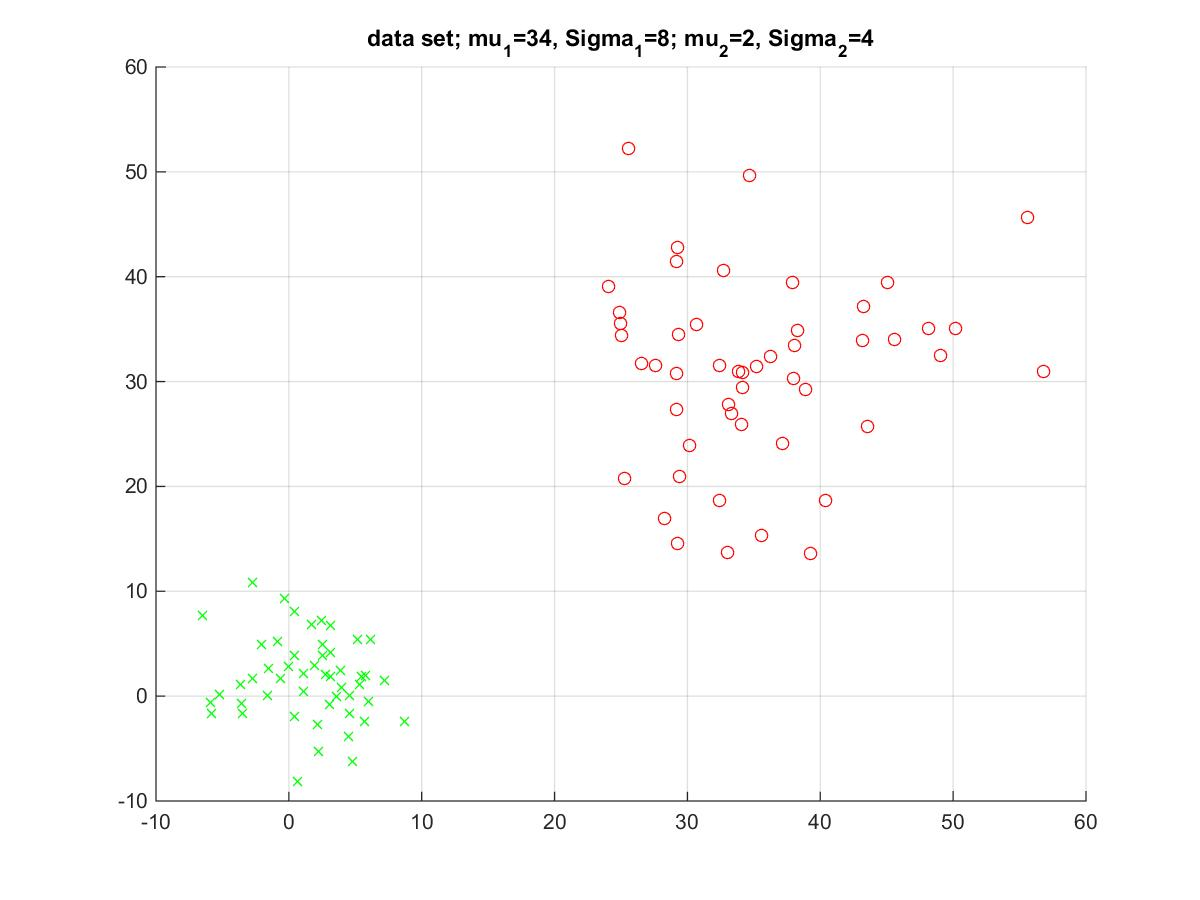
\includegraphics[width=0.4\textwidth]{./images/DataSet_200.jpg} \\
 & \\
\hline
 & \\
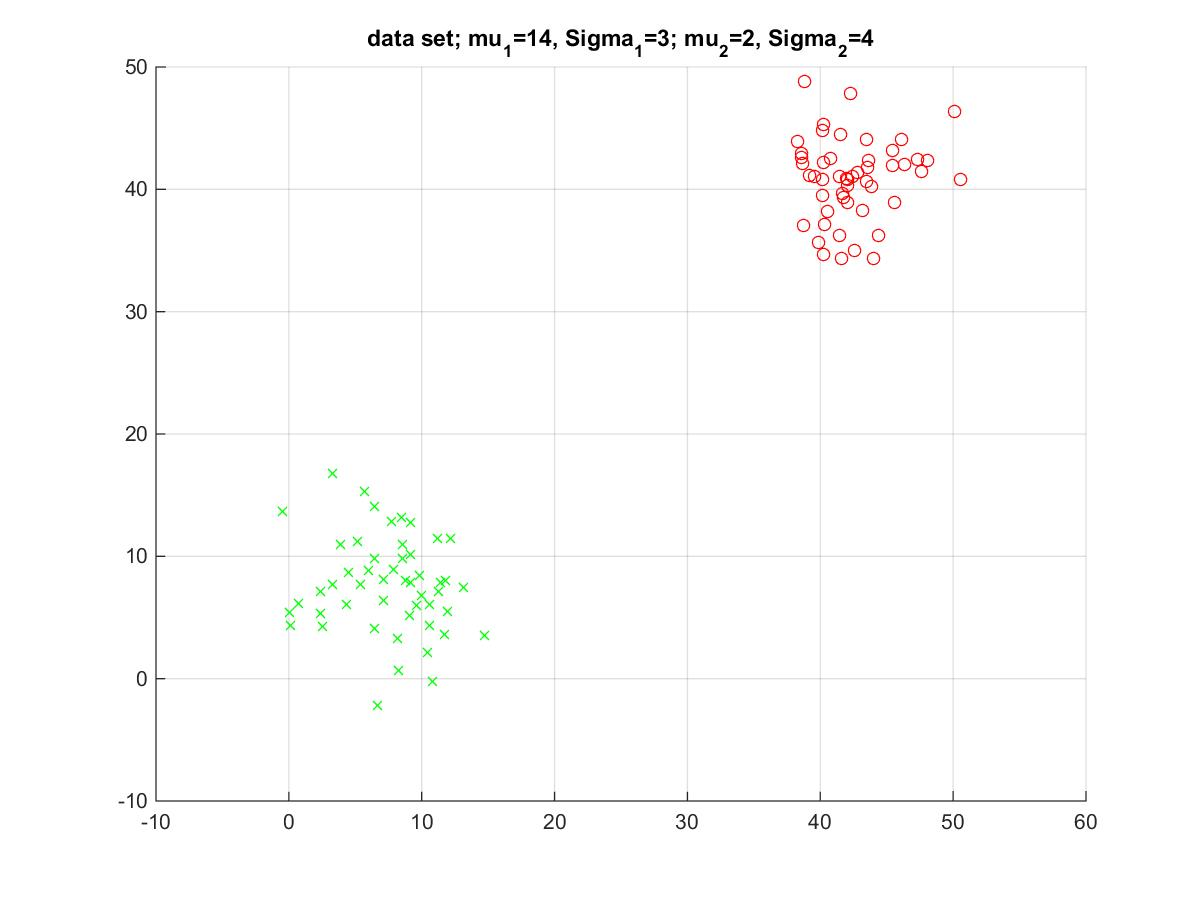
\includegraphics[width=0.4\textwidth]{./images/DataSet_300.jpg} & 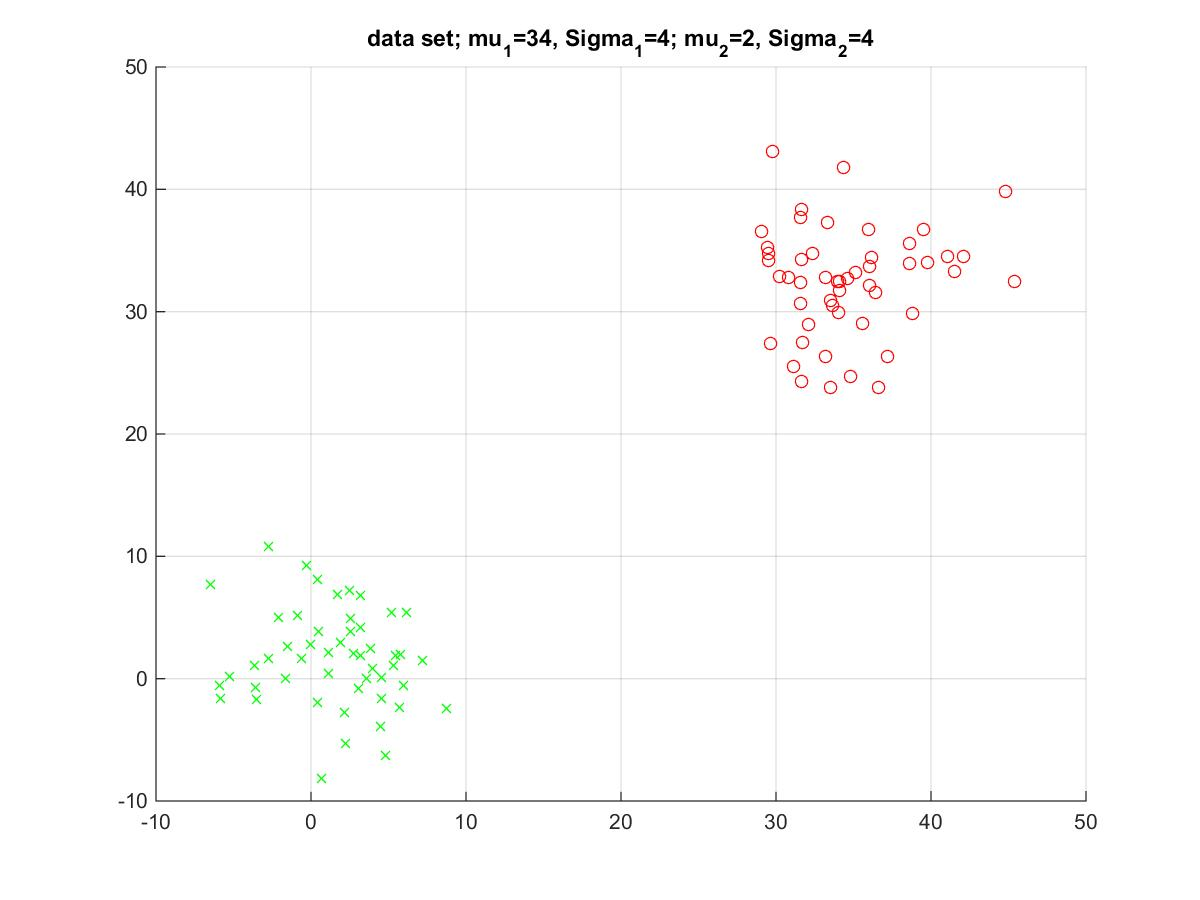
\includegraphics[width=0.4\textwidth]{./images/DataSet_400.jpg} \\
 & \\
\hline
\end{tabular}
\caption{Iteration distribution over gamma}
\label{tab:DataSets}
\end{table}

\chapter{Einfaches Perceptron - Perceptrontraining}

\section{Anzahl Iterationen}

Die Anzahl der Iterationen h\"angt ma{\ss}geblich von der \emph{margin} der separierbaren Daten ab. Je kleiner die margin, das hei{\ss}t der Minimalabstand zwischen den beiden Mengen, desto mehr Iterationen sind notwendig, bis der Algorithmus terminiert. Dies ist aus der Angabe der Iterationen aus ~\ref{tab:DataSetsAndBounds} ersichtlich.


\section{Welchen Einflu{\ss} hat die Schrittweite}

Der Einflu{\ss} der Schrittweite h\"angt sowohl von den Eingangsdaten als auch vom gew\"ahlten Algorithmus ab.
Es ist zu beobachten, da{\ss} der batch-Algorithmus keine gro{\ss}en Abweichungen zeigt, egal welches $\gamma$ gew\"ahlt wird. Beim online-Verfahren ist der Einflu{\ss} gr\"o{\ss}er, das hei{\ss}t die Varianz in den ermittelten Iterationen ist h\"oher, aber auch hier ist kein eindeutiger Bereich \"uber alle Simulationen auszumachen, wo ein gegebenes $\gamma$ die Iterationen des Algorithmus wesentlich reduziert. Zu sehen ist die Verteilung der Iterationen \"uber ein $\gamma$ von 0.1 bis 4 f\"ur die jeweiligen unterschiedlichen Datens\"atze in Tabelle ~\ref{tab:GammaToIterations}.

\begin{table}[h]
\begin{tabular}{| c | c |}
\hline
 & \\
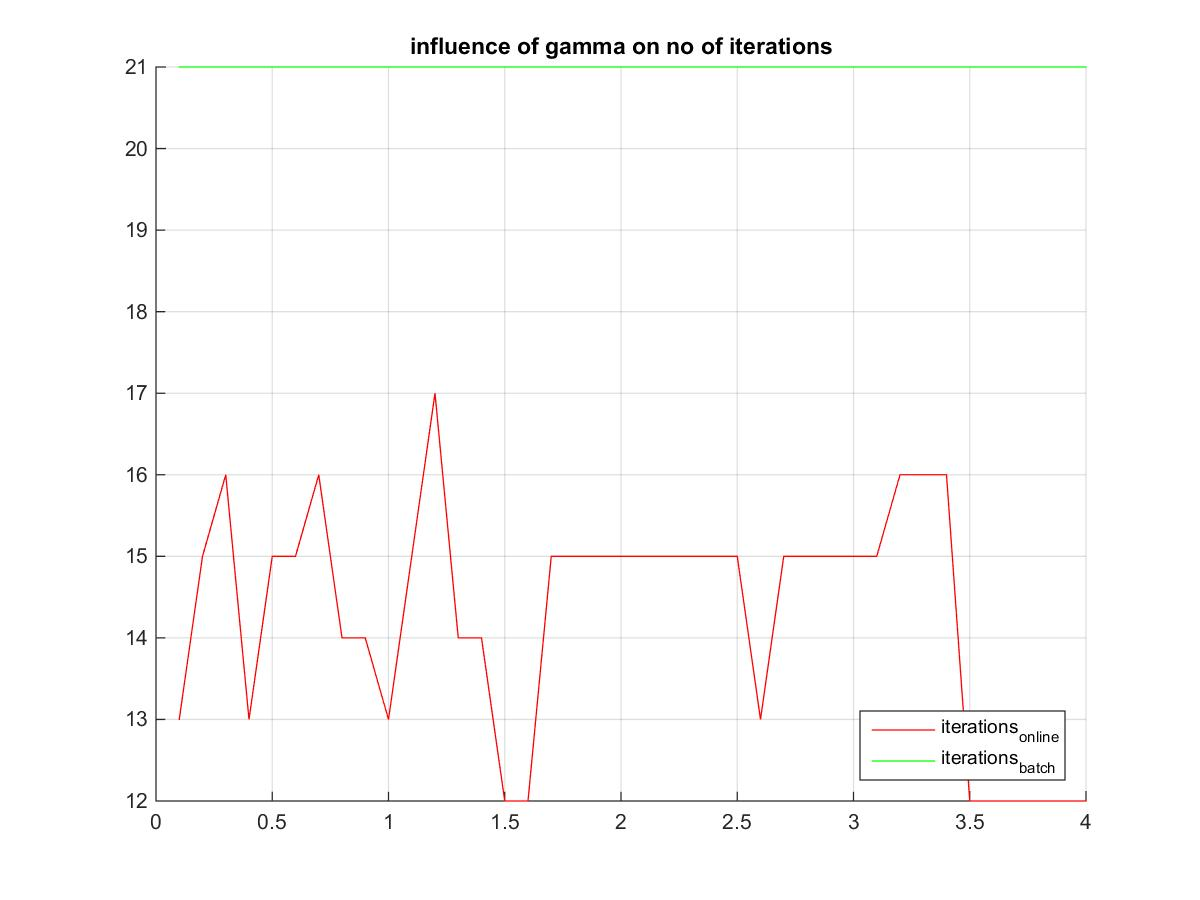
\includegraphics[width=0.4\textwidth]{./images/GammaToIterations_0150.jpg} & 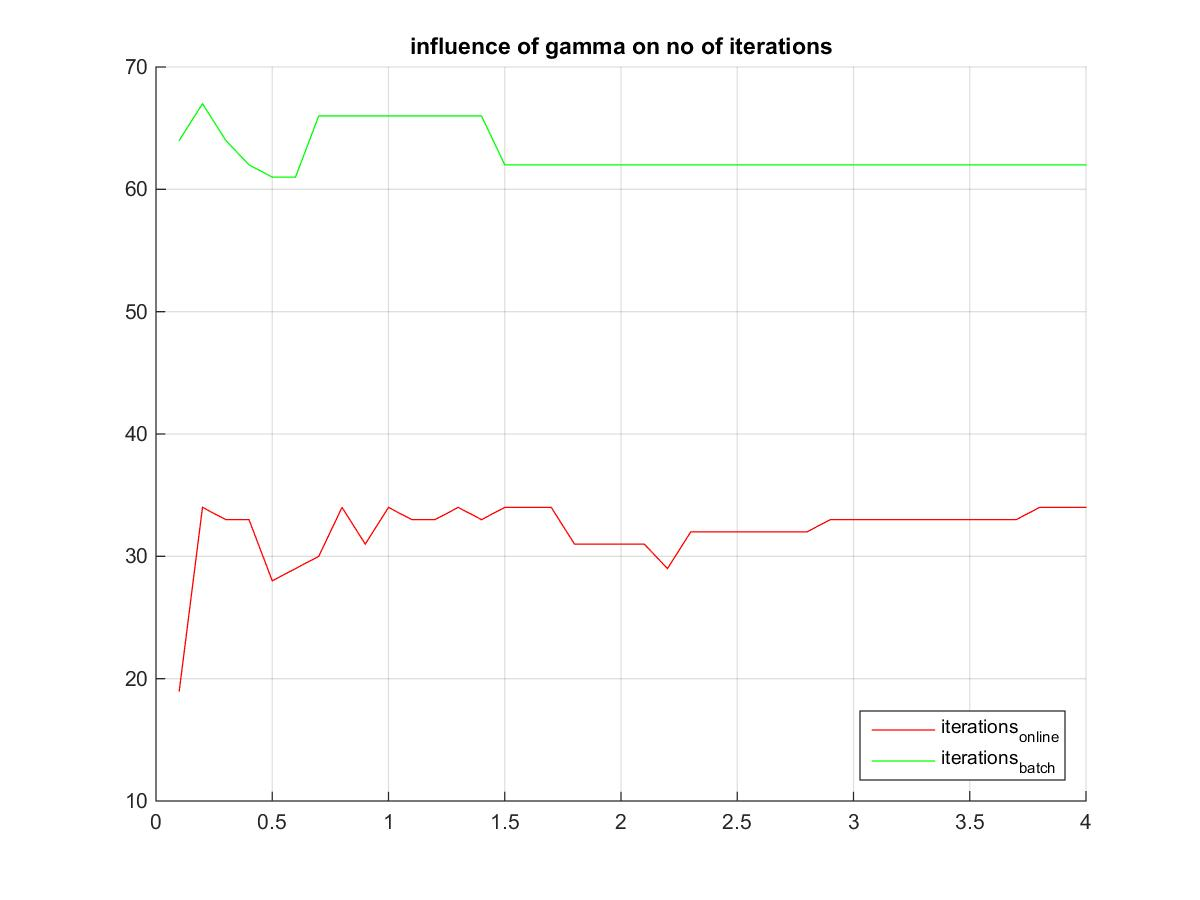
\includegraphics[width=0.4\textwidth]{./images/GammaToIterations_0250.jpg} \\
 & \\
\hline
 & \\
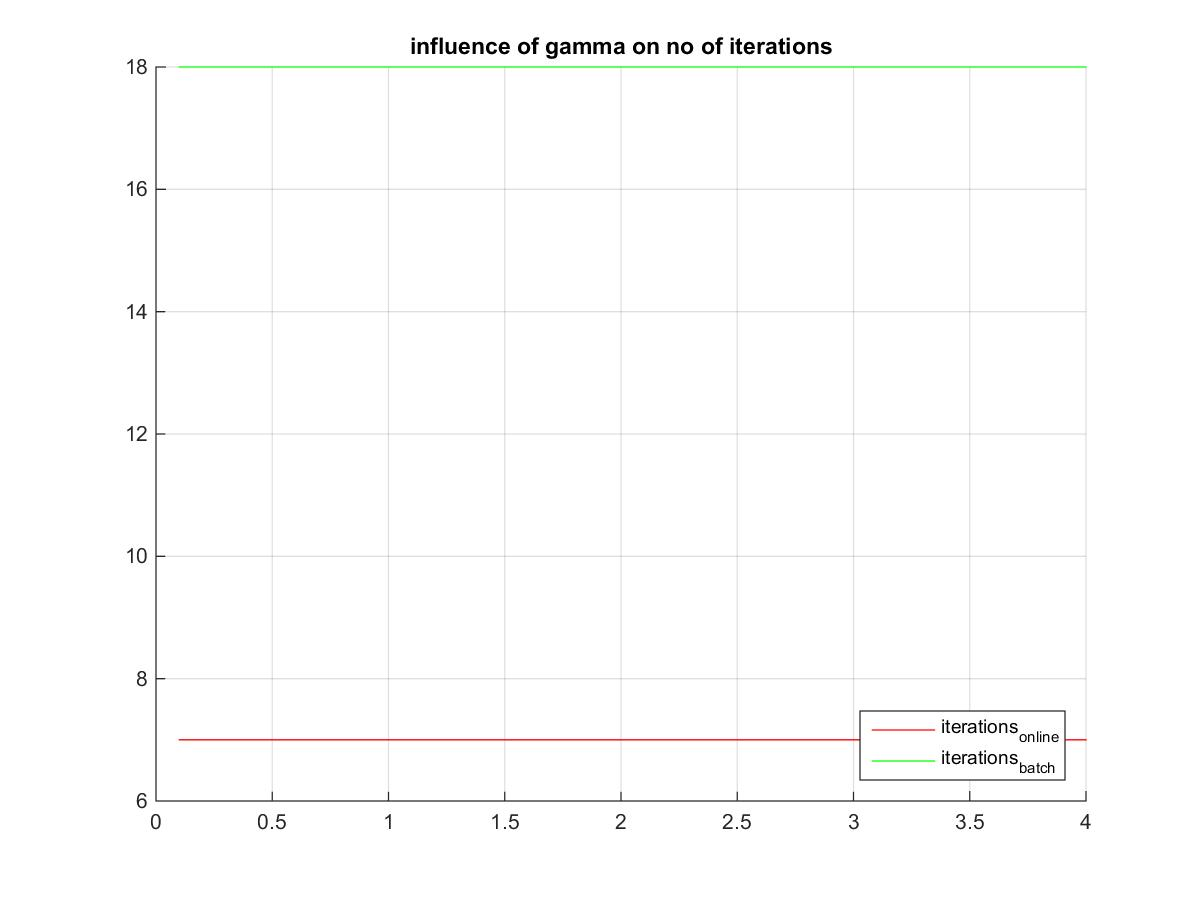
\includegraphics[width=0.4\textwidth]{./images/GammaToIterations_0350.jpg} & 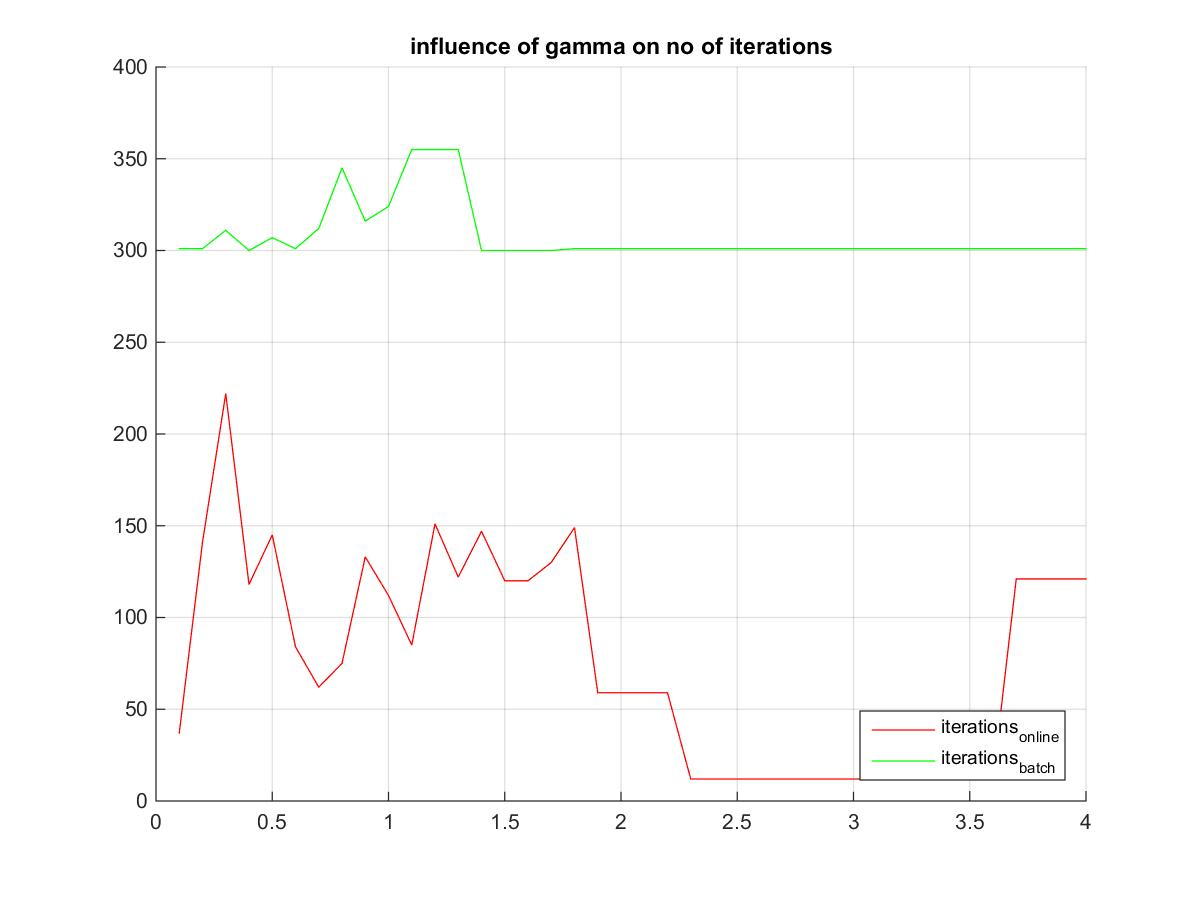
\includegraphics[width=0.4\textwidth]{./images/GammaToIterations_0450.jpg} \\
 & \\
\hline
\end{tabular}
\caption{iteration distribution over gamma}
\label{tab:GammaToIterations}
\end{table}


\section{Daten und Entscheidungsgrenzen im $\mathbb{R}^2$}

Die ermittelten Entscheidungsgrenzen des batch-learning sowie des online-learning Algorithmus sind f\"ur die einzelnen Datens\"atze und ein gegebenes $\gamma$ von 1 in Tabelle ~\ref{tab:DataSetsAndBounds} zu sehen.

\begin{table}[h]
\begin{tabular}{| c | c |}
\hline
 & \\
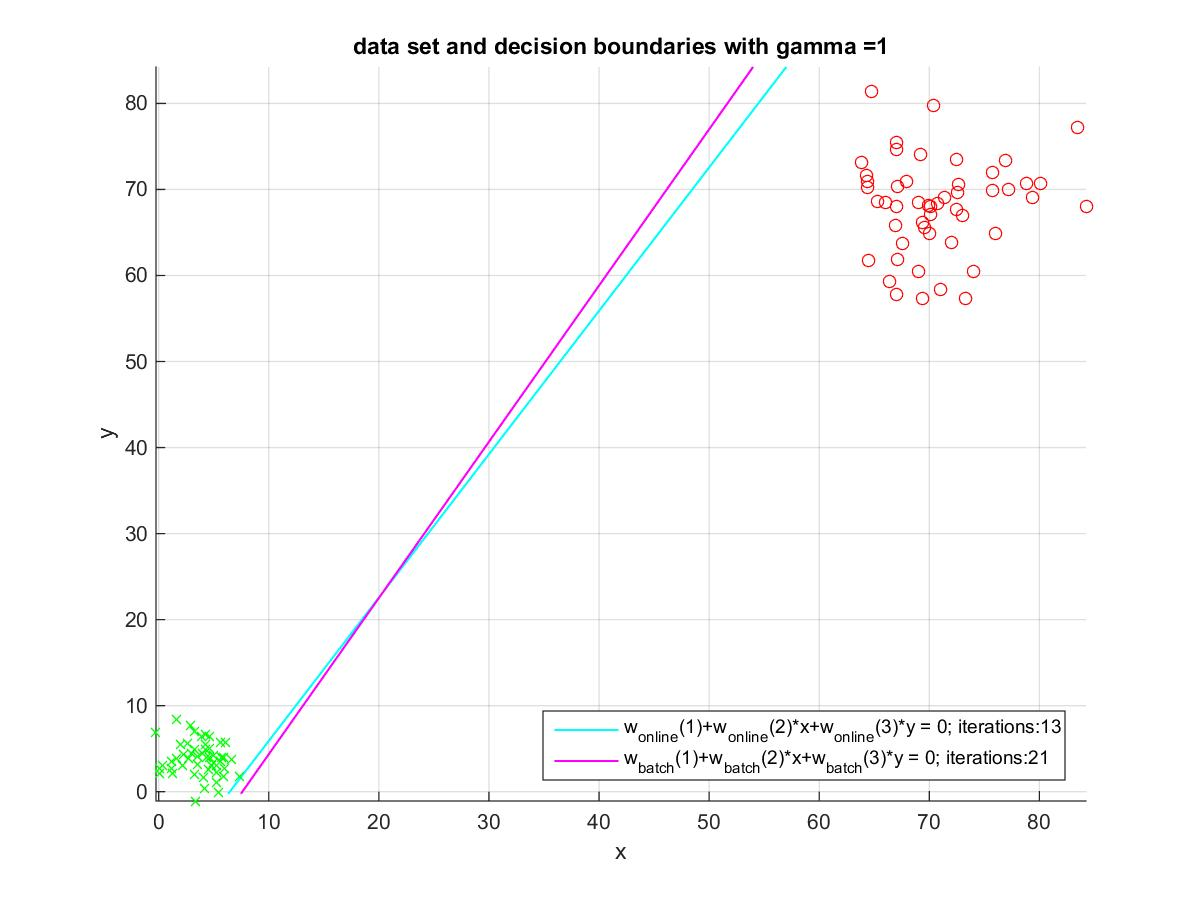
\includegraphics[width=0.4\textwidth]{./images/DataSetAndDecisionBoundary_110.jpg} & 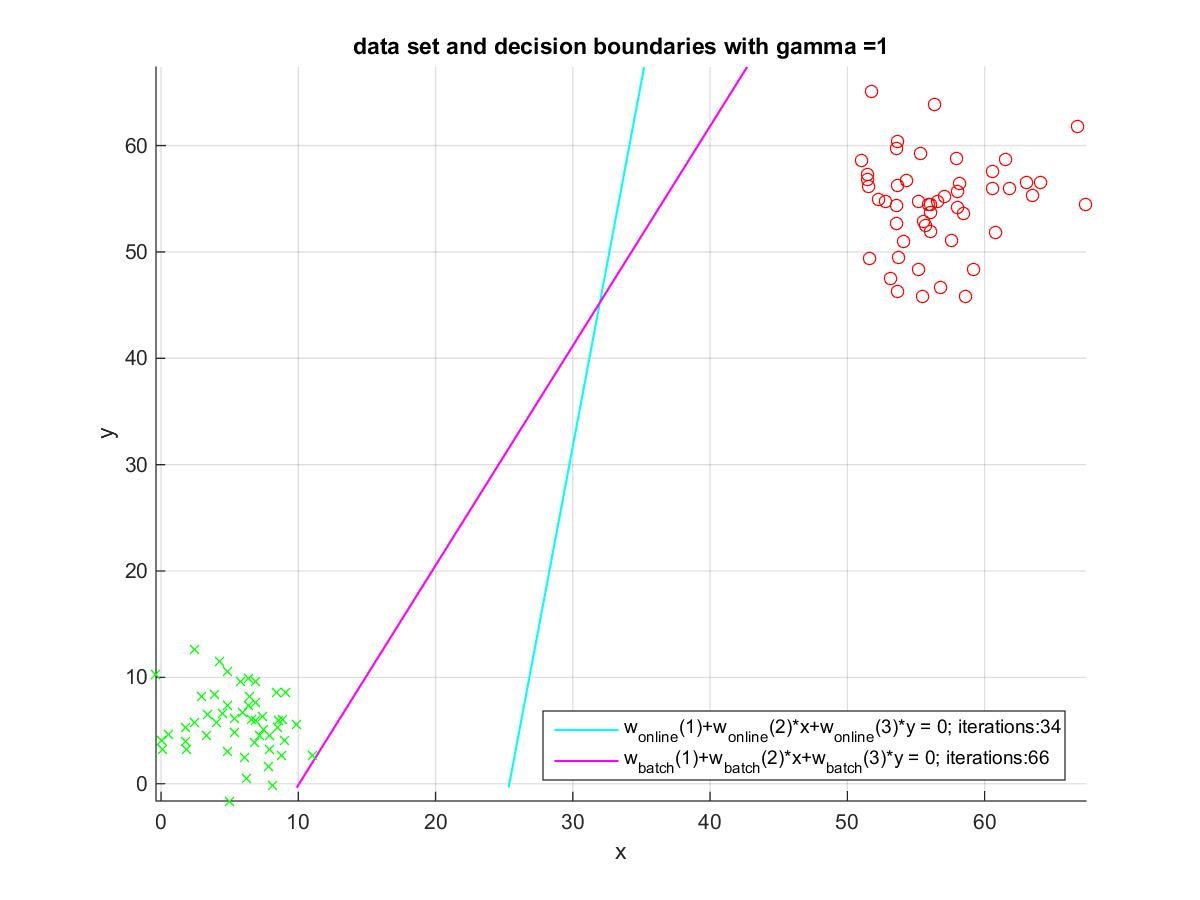
\includegraphics[width=0.4\textwidth]{./images/DataSetAndDecisionBoundary_210.jpg} \\
 & \\
 $set_{1}$: $\mu_1=10$, $\Sigma_1=5$ & $set_{1}$: $\mu_1=10$, $\Sigma_1=4$ \\
 $set_{2}$: $\mu_2=2$, $\Sigma_2=2$ & $set_{2}$: $\mu_2=2$, $\Sigma_2=3$ \\
\hline
 & \\
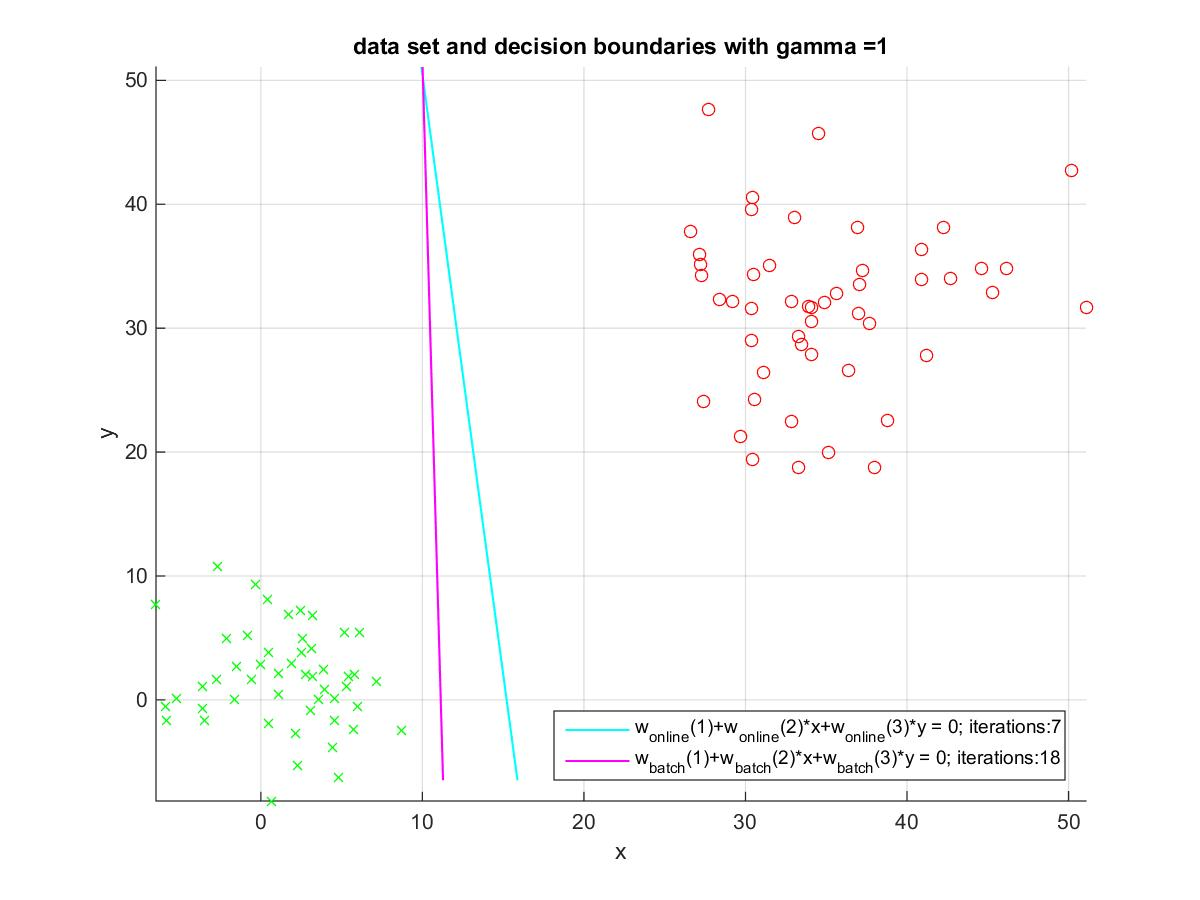
\includegraphics[width=0.4\textwidth]{./images/DataSetAndDecisionBoundary_310.jpg} & 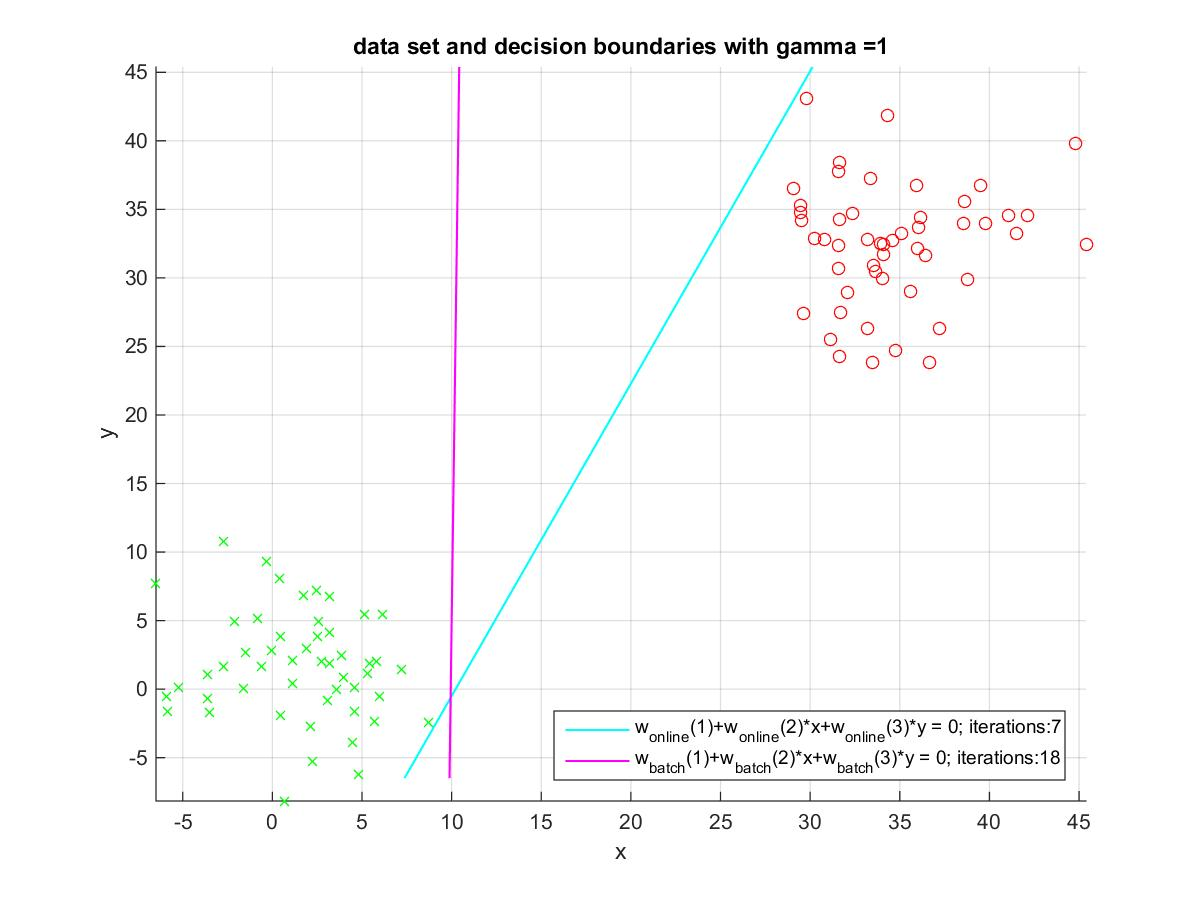
\includegraphics[width=0.4\textwidth]{./images/DataSetAndDecisionBoundary_410.jpg} \\
 & \\
$set_1$: $\mu_1=10$, $\Sigma_1=3$ & $set_1$: $\mu_1=10$, $\Sigma_1=2$ \\
$set_2$: $\mu_2=2$, $\Sigma_2=4$ & $set_2$: $\mu_2=2$, $\Sigma_2=5$ \\
\hline
\end{tabular}
\caption{iteration distribution over gamma}
\label{tab:DataSetsAndBounds}
\end{table}

\section{Wie ist das Verhalten bei nicht linear separierbaren Daten}

Der Algorithmus terminiert nicht da bei jedem Durchlauf Daten gefunden werden, welche in der falschen Klasse landen.

\chapter{Lineare Regression}

Wir erstellen Daten im Bereich von $[0,5]$ mit einer Schrittweite von 0.1 aus der Funkion:

\begin{equation}
y=x^2-Gx+1
\end{equation}

Des weiteren erstellen wir eine Trainingsmenge aus jedem sechsten Datenpunkt und f\"ugen je einen Zufallswert aus $N(\mu=0,\Sigma=0.7)$ hinzu.

\section{Gewichtsvektor mittels Gradientenabstieg bei quadratischer Fehlerfunktion}

TODO: depend on valid online LMS!

\section{Optimaler Gewichtsvektor $w^*$}

Den optimalen Gewichtsvektor $w^*$ kann man \"uber die Bestimmung der Pseudoinversen $A^+$ f\"ur die Gleichung $Aw^*=b$ ermitteln.
Die Gleichung $w^*=A^+b$ bestimmt das optimale $w^*$. 
Dabei berechnet sich $A^+$ wie folgt:

\begin{eqnarray}
A^+ =& (AA^T)^{-1} &\textnormal{ f\"ur invertierbare } AA^T \\
A^+ =& (AA^T)^{-1} + \lambda I &\textnormal{ f\"ur nicht invertierbare} AA^T \textnormal{ mit } \lambda<<1
\end{eqnarray}

Das ermittelte Ergebnis f\"ur $w^*$ mit normalisierten Daten aus dem $\mathbb{R}^2$ lautet: $w^*=(1.0106678, - 10.0086, 1.8960336, 0.0262634)$.

\section{Konvergenzverhalten in Abh\"angigkeit von $\gamma$}

TODO: depend on valid online LMS!

In Figur ~\ref{fig:ConvergenceOverGamma} ist zu sehen, da{\ss} die Anzahl der notwendigen Iterationen um zu einem Optimum zu gelangen mit der Gr\"o{\ss}e von $lambda$ exponentiell abnimmt, bis es sich auf einem fixen Wert einpendelt.

\begin{figure}[h]
\centering
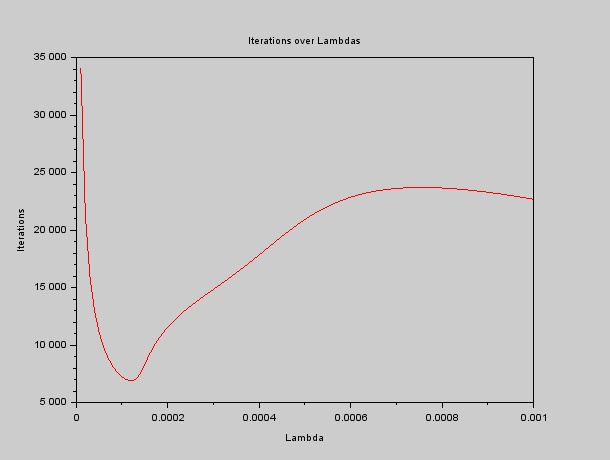
\includegraphics[width=0.4\textwidth]{./images/ConvergenceOverGamma.jpg} \\
\caption{convergence over gamma}
\label{fig:ConvergenceOverGamma}
\end{figure}

\section{Erwartungswert und Varianz von $w^*$ im Bezug zu Dimensionalität $d$ von $f(x)$}

Erwartungswert und Varianz von $w^*$ im Bezug zu Dimensionalität $d$ von $f(x)$ zeigt, dass je h\"oher die Dimensionalität $d$ steigt, desto h\"oher auch die Varianz $Sigma$ der ermittelten Werte f\"ur $w^*$ f\"ur verrauschte Eingangsdaten wird. Dies ist auch klar, da höherdimensionale Koeffizienten von $w^*$ h\"ohere Frequenzen repr\"asentieren, welche durch das Verrauschen der Eingangsdaten st\"arker betroffen sind als niedrigere Frequenzen.
Interessanterweise steigt die Varianz aller Koeffizienten von $w^*$ in Tabelle ~\ref{tab:VarianceAndDeviantion} nur bis zu einer Dimensionalit\"at des Problems von 6, danach f\"allt sie wieder. Es ist aber anzunehmen, dass dies zum Einen aufgrund von Unzul\"anglichkeiten beim generieren der Pseudoinversen zur Berechnung von $w^*$ liegt und zum Anderen von der fehlenden Betrachunng noch h\"oherer Dimensionen, wo sich globale Anstieg der Varianz sicherlich fortsetzt.

\begin{table}[h]
\begin{tabular}{| c | c |}
\hline
 & \\
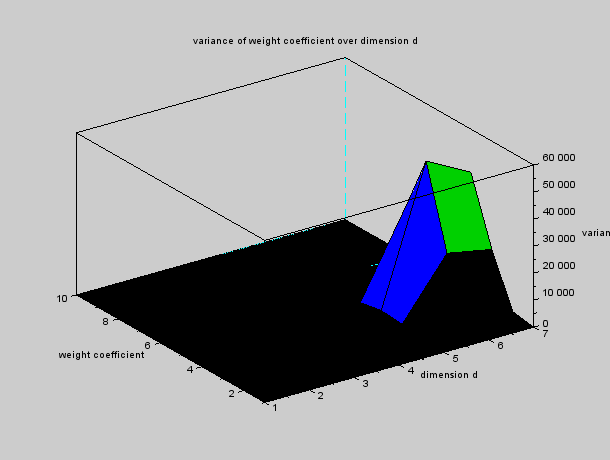
\includegraphics[width=0.4\textwidth]{./images/VarianceWeightCoeffinientsOverDimension.png} & 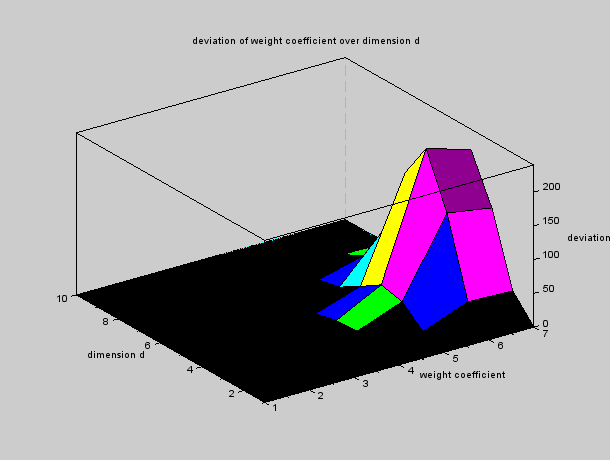
\includegraphics[width=0.4\textwidth]{./images/DeviationWeightCoeffinientsOverDimension.png} \\
 & \\
variance of weight coeffinients & deviation of weight coeffinients \\
\hline
\end{tabular}
\caption{variance and deviantion of $w^*$ over dimension}
\label{tab:VarianceAndDeviantion}
\end{table}

Des weiteren ist in Figur ~\ref{fig:Overfitting} festzustellen, dass f\"ur h\"oherdimensionale Komponenten f\"ur $w^*$ durch overfitting der Kurve $f(x)$ die Varianz zunimmt, zu sehen in den Schwingungen der Kurven.

\begin{figure}[h]
\centering
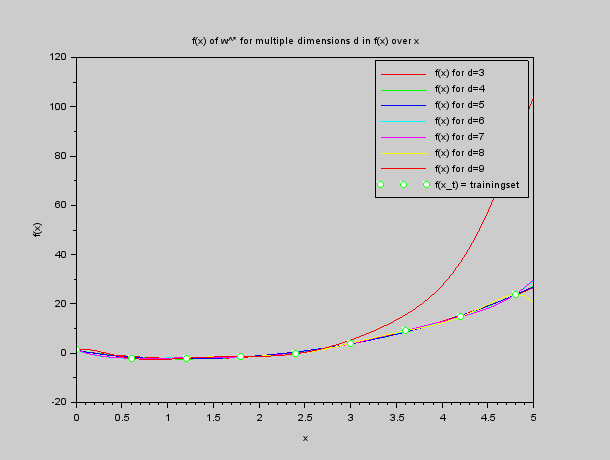
\includegraphics[width=0.4\textwidth]{./images/f_x_w_star_overDimensions.png} \\
\caption{overfitting of $f_{w^*}(x)$ curves over dimension}
\label{fig:Overfitting}
\end{figure}

\section{Mittlere quadratische Abweichung von $f_{w^*}(x^*)$}

Wie erwartet, steigt auch die mittlere quadratische Abweichung von $f_{w^*}(x^*)$ mit der Zunahme der Dimension $d$ an, wie in Figur ~\ref{fig:MeanError} zu sehen ist.

\begin{figure}[h]
\centering
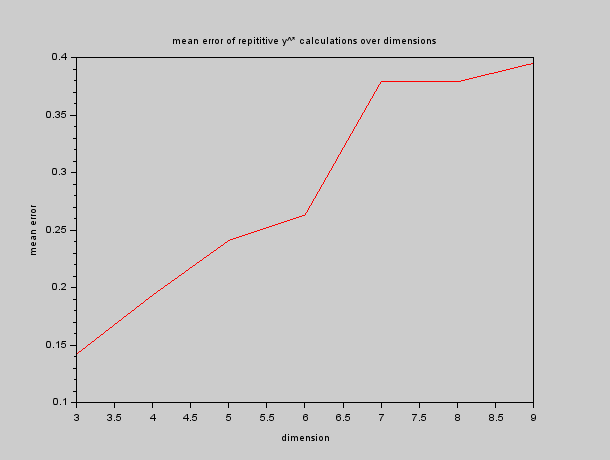
\includegraphics[width=0.4\textwidth]{./images/MeanErrorOverDimensions.png} \\
\caption{mean error of $f_{w^*}(x^*)$ curves over dimension}
\label{fig:MeanError}
\end{figure}

\section{Gewichtsvektor $w^*$ bei ungest\"orter Trainingsmenge \"uber Dimension $d$}

Die resultierenden Kurven f\"ur $f_{w^*}(x)$ welche aus der ungest\"orten Trainingsmenge ermittelt wurden fitten die Originalpunkte aus der Originalkurve $y = 2x^2-Gx+1$ naturgem\"a{\ss} wesentlich besser als die Kurven, welche auf der verrauschen Trainingsmenge basieren. Dies ist in Tabelle ~\ref{tab:f_x_overDimension} zu sehen. Der Ausrei{\ss}er bei Dimension $9$ ist wiederum auf Schw\"achen in der Bestimmung der Pseudoinversen zur\"uckzuf\"uhren.

\begin{table}[h]
\begin{tabular}{| c | c |}
\hline
 & \\
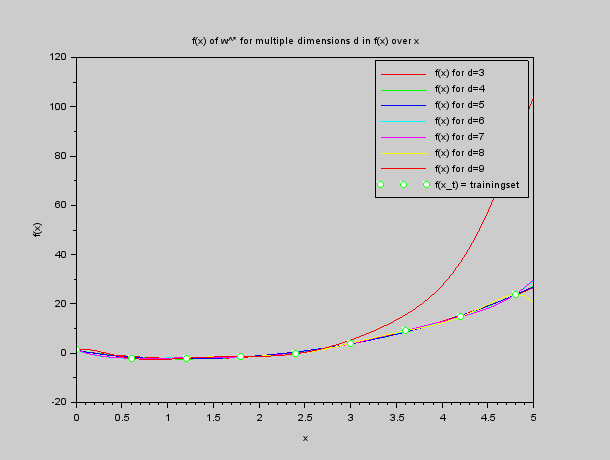
\includegraphics[width=0.4\textwidth]{./images/f_x_w_star_overDimensions.png} & 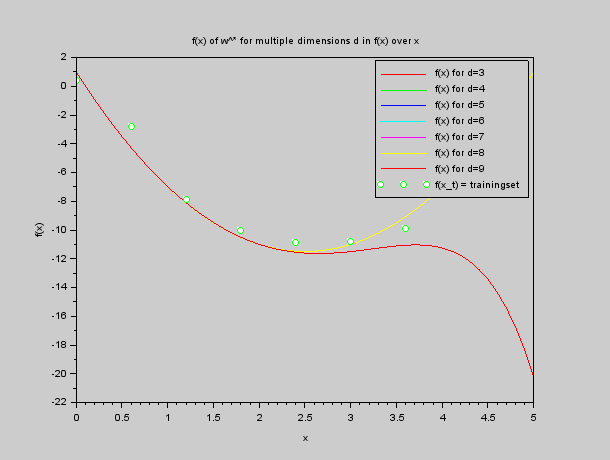
\includegraphics[width=0.4\textwidth]{./images/f_x_w_star_not_preturbed_overDimensions.png} \\
 & \\
$w^*$ based on preturbed trainingsset & $w^*$ based on not preturbed trainingsset \\
\hline
\end{tabular}
\caption{$f_{w^*}(x)$ over dimension}
\label{tab:f_x_overDimension}
\end{table}


\end{document}          
